\documentclass[a4paper]{article}
\usepackage{amsmath,amssymb,caption,float,graphicx,minted,xcolor}
\usepackage[utf8]{inputenc}
\usepackage[english]{babel}
% \usepackage[backend=bibtex]{biblatex}
% \addbibresource{Lab3.bib}
\captionsetup[figure]{labelsep=period}
\definecolor{bg}{rgb}{0.95,0.95,0.95}
\renewcommand\thesection{\arabic{section}}
\usemintedstyle{emacs}
\begin{document}
\begin{center}
    \huge
    \textbf{VE482\\Introduction to Operating Systems\\}
    \Large
    \vspace{15pt}
    \uppercase{\textbf{Homeork 2}}\\
    \large
    \vspace{5pt}\today\\
    \vspace{5pt}
    Yihua Liu 518021910998
    \vspace{5pt}
    \rule[-5pt]{.97\linewidth}{0.05em}
\end{center}
\section*{Ex. 1 — Multiprogramming}
A few years ago when computers featured less RAM it is was common to increase it in order to enhance CPU performance. In order to better understand the link between the two we now create a simple model for multiprogramming. We assume all the processes to be similar and spending the same fraction $p$ of their time waiting for Input/Output (I/O) to complete.
\begin{enumerate}
    \item What is the probability for $n$ processes to be waiting at the same time, then express the CPU utilisation as a function of $n$?\\
    The probability for $n$ processes to be waiting at the same time is $p^n$.\\
    The CPU utilisation as a function of $n$ is $1-p^n$.\\
    \item Sketch the curve representing the CPU utilisation as a function of the number of processes for the following values of $p$: 25\%, 60\% and 90\%.
    \begin{figure}[H]
        \centering
        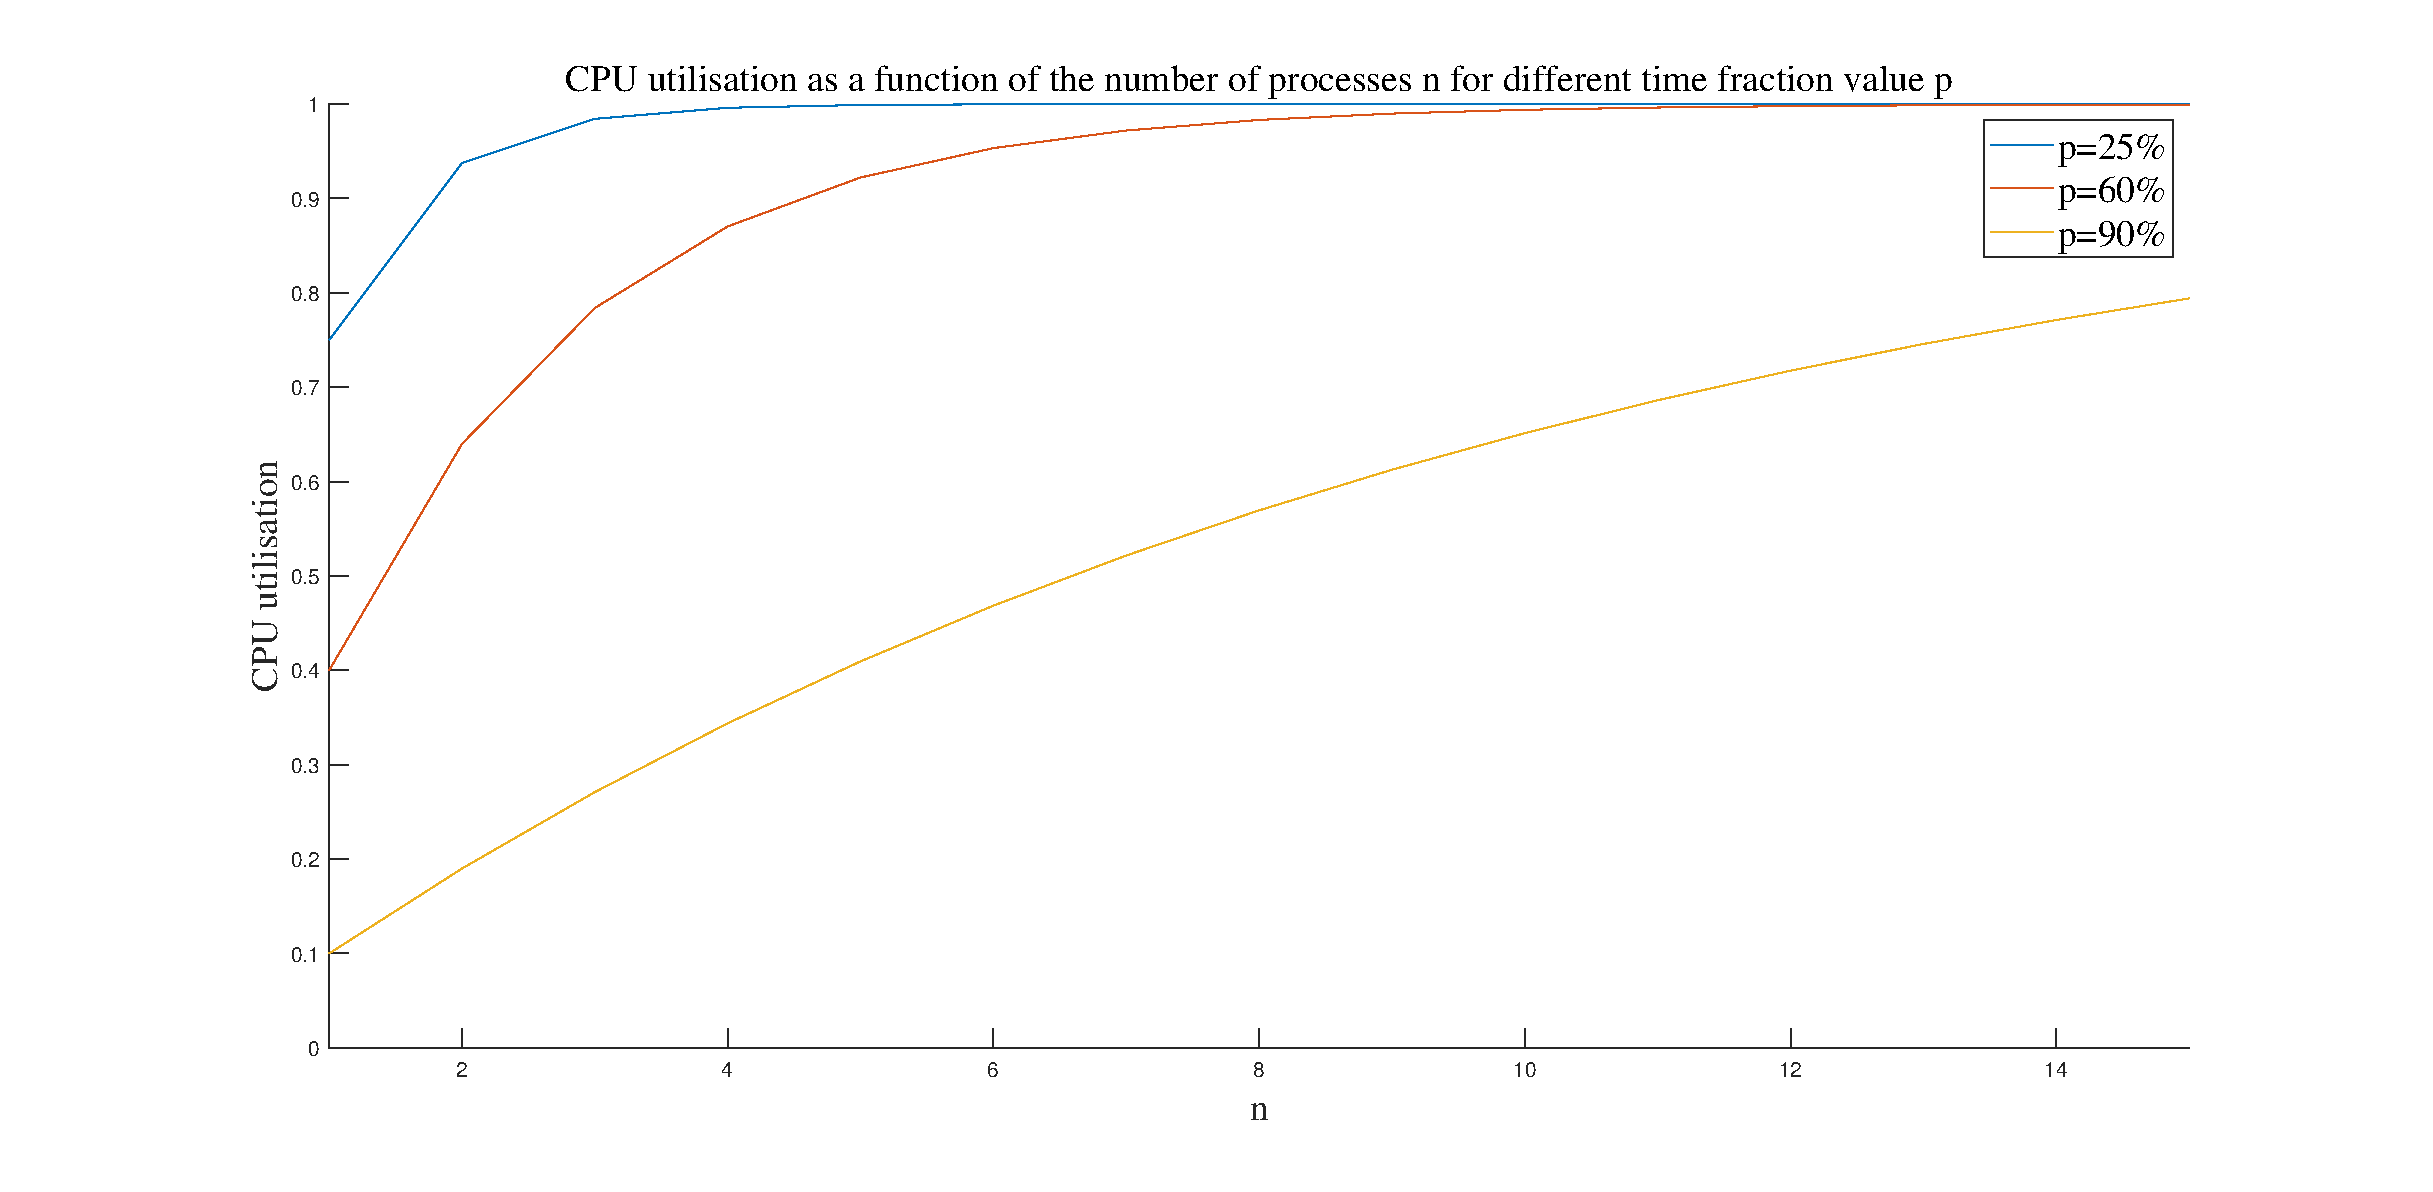
\includegraphics[width=1\textwidth]{1.eps}
        \caption{CPU utilisation as a function of the number of processes $n$ for different time fraction value $p$.}
    \end{figure}
    \item A certain old computer has 256 MB of RAM, once loaded a light operating system uses 96 MB of RAM. Several programs are launched each of them using 48 MB.
    \begin{enumerate}
        \item How many processes can be store simultaneously in memory?\\
        \[(256-48)/48=3.\]
        3 processes can be store simultaneously in memory.
        \item Assuming an average of 90\% I/O waiting time what is the CPU utilisation?\\
        \[1-0.9^3=0.271=27.1\%.\]
        The CPU utilisation is 27.1\%.
        \item What is the effect of adding 256 MB, 512 MB and 1024 MB of RAM. Argue on which amount would be the most beneficial and would be worth the investment.\\
        % Original: Number of simultaneous processes is $n=(256-48)/48=3$, CPU utilisation is $1-0.9^3\approx27.1\%$, each program uses 9.03\%.\\
        We assume for the three RAMs, the price per MB is the same. To choose the most beneficial one, we need to consider costs, which can be measured in CPU utilisation per 256 MB that are added.
        Adding 256 MB: Number of simultaneous processes is $n=\lfloor(512-96)/48\rfloor=8$, CPU utilisation is $1-0.9^8\approx56.95\%$, efficiency improved by 56.95 - 27.1\% = 29.85\% per 256 MB that are added.\\  % each program uses 7.12\%
        Adding 512 MB: Number of simultaneous processes is $n=(768-96)/48=14$, CPU utilisation is $1-0.9^{14}\approx77.12\%$, efficiency improved by (77.12\% - 27.1\%) / 2 = 25.01\% per 256 MB that are added.\\
        Adding 1024 MB: Number of simultaneous processes is $n=\lfloor(1280-96)/48\rfloor=24$, CPU utilisation is $1-0.9^{24}\approx92.02\%$, efficiency improved by (92.02\% - 27.1\%) / 4 = 16.23\% per 256 MB that are added.\\  % each program uses 3.83\%
        Therefore, adding 256 MB would be most beneficial and would be worth the investment.
    \end{enumerate}
\end{enumerate}
\section*{Ex. 2 — Keymap in Minix 3}
Map the Shit+F7 key to displaying how many processes are currently running.\\
This can be achieved following the steps:\\
\begin{enumerate}
    \item Find all the files that need to be modified;\\
    \texttt{/usr/src/servers/is/dmp.c}, \texttt{/usr/src/servers/is/proto.h}, \texttt{/usr/src/servers/is/dmp\_kernel.c}.
    \item Locate the part of the code that should be updated;\\
    At Line 33 of \texttt{/usr/src/servers/is/dmp.c}, at Line 21 of \texttt{/usr/src/servers/is/proto.h}, at the end of \texttt{/usr/src/servers/is/dmp\_kernel.c}.
    \item Check how to process table is stored;
    \item Count the number of running processes;

    At Line 21 of \texttt{/usr/src/servers/is/proto.h}, add one line:
    \begin{minted}[frame=single,bgcolor=bg,breaklines,linenos]{c}
    void procnum_dmp(void);
    \end{minted}
    \begin{figure}[H]
        \centering
        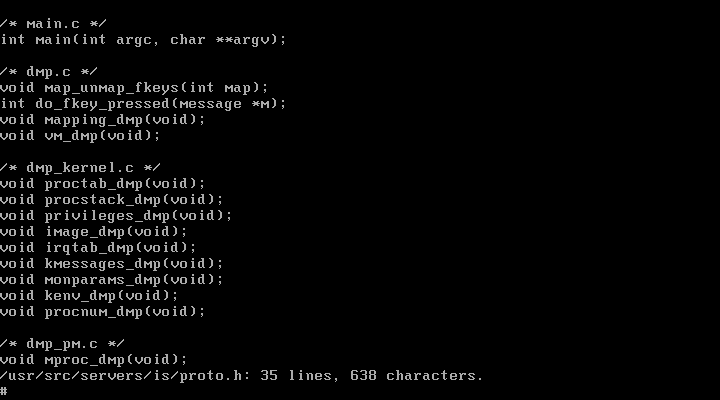
\includegraphics[width=1\textwidth]{3.png}
    \end{figure}
    At the end of \texttt{/usr/src/servers/is/dmp\_kernel.c}, add a function:
    \begin{minted}[frame=single,bgcolor=bg,breaklines,breakanywhere,linenos]{c}
    /*===========================================================================*
     *				procnum_dmp  				     *
     *===========================================================================*/
    void procnum_dmp()
    {
      register struct proc *rp;
      int r,n=0;
    
      /* First obtain a fresh copy of the current process table. */
      if ((r = sys_getproctab(proc)) != OK) {
        printf("IS: warning: couldn't get copy of process table: %d\n", r);
        return;
      }
    
      for (rp=BEG_PROC_ADDR; rp<END_PROC_ADDR; rp++) {
          if (isemptyp(rp))
            continue;
          n++;
      }
    
      printf("Number of currently running processes is %d\n", n);
    }
    \end{minted}
    \begin{figure}[H]
        \centering
        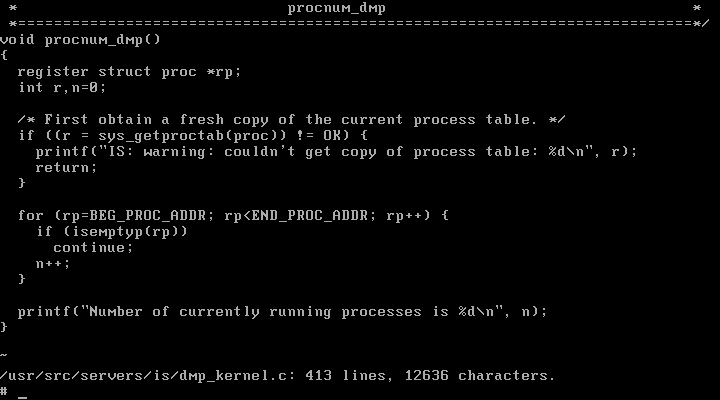
\includegraphics[width=1\textwidth]{4.png}
    \end{figure}
    \item Map the newly written function to the Shift-F7 key;
    At Line 33 of \texttt{/usr/src/servers/is/dmp.c}, add one line:
    \begin{minted}[frame=single,bgcolor=bg,breaklines,linenos]{c}
    { SF7,  procnum_dmp, "Print number of currently running processes" },
    \end{minted}
    \begin{figure}[H]
        \centering
        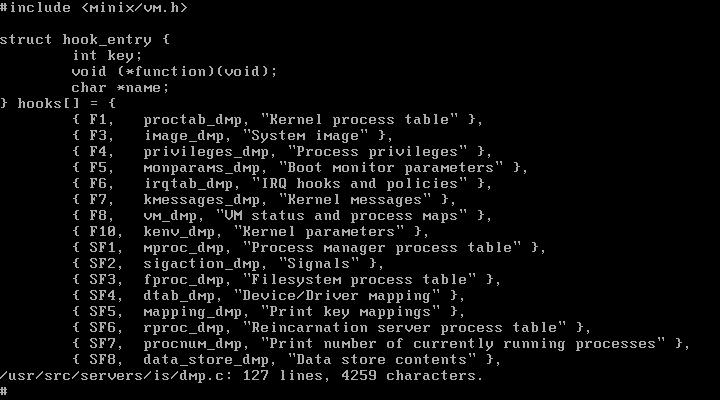
\includegraphics[width=1\textwidth]{2.png}
    \end{figure}
    \item Recompile the kernel and test.
    \begin{minted}[frame=single,bgcolor=bg,breaklines,linenos]{bash}
        cd /usr/src
        make build && reboot  # remember to reboot
    \end{minted}
\end{enumerate}
\begin{figure}[H]
    \centering
    
\includegraphics[width=1\textwidth]{5.png}
\end{figure}
\begin{figure}[H]
    \centering
    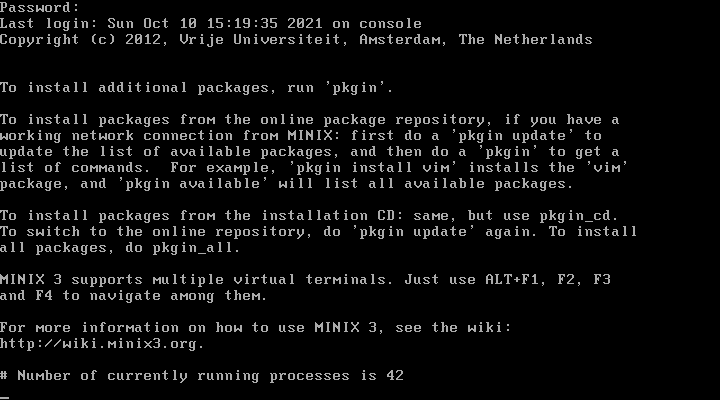
\includegraphics[width=1\textwidth]{6.png}
\end{figure}
\end{document}